\chapter{Introduction}
\section{Motivation}

Data visualisation is turning out to be an indispensable subject for our generations. Advancing information technology allows for the collection and management of increasing amounts of even more complex data. However, in order to understand the motivation for presenting data graphically, it is helpful to look at its early origins.

With the ability of humans to communicate through language and signs, the need to visualise data emerged. The availability of different media has always decided what results look like and whether they still exist today. An early example of preserved data visualisation among others is Turin's Papyrus Map. The medium papyrus was used for records of typographical interests in ancient Egypt \citep{harrell1992}. Because of its long durability, the map still exists today and can deliver rich information. For example can some perception criteria that are discussed later already be found in the artwork.

As information processing and means of illustration develop, new possibilities and challenges arise. Today, a broad repertoire of approaches can be used for visualisations. Still, regardless of the application, the quality of a model can only be assessed in the context of its intention and the observer. When facing a very simplistic graph it might fit perfectly for someone that is only interested in getting a brief understanding on the underlying data. In this case, the visualisation works out great even though only few of the data is transformed into information. A variety of methods holds both the opportunity for suitable as well as the risk of detrimental representation. Basic goals besides adequate visualisation are traceability and reproducibility. To ensure this, reconstructable instructions often are published as well as the data they operate on. Motivated by this, the data, code, and results of this work are publicly available at \url{https://github.com/robinkillewald/DV-Seminar-Thesis}.

In this paper, the Internet Movie Database is introduced and its content and structure is described. After that, a theoretical background upon which further visualisations will be based is laid. This involves explanations of the contexts in which data and information occur, the approximation of approaches derived from literature for measuring the quality of graphics, their differentiation and assessment within different facets of perception as well as methods to visualise data. The theoretical part is followed by a comparison that involves the described criteria and methods that get applied to different types of data followed by an evaluation of results and an outlook in further directions. 

\section{The Internet Movie Database}

The Internet Movie Database's origins are based on few film fan. When the Internet enabled sharing information on portals or bullet boards, many first-of-a-kind discussions developed into own portals. In IMDb's case, a few movie enthusiasts sharing lists of actors in 1990 developed in what we now know as the biggest database for motion picture. Starting with actresses that have beautiful eyes, the lists developed and merged into a larger database. Already in early days, one of the goals was to keep completing the lists while not missing any entries or movies. With the addition of shell scripts to access and filter the data, the database was first known as ''rec.arts.movies movie database''. Later in 1993, it got hosted as ''Cardiff Internet Movie Database'' by the Cardiff University in Wales. Over the time, there were added new categories, ratings and submissions via mail. 

1996 marks the first year that the IMDb was incorporated. After being subject to Col Needham's Internet Movie Database Ltd., Amazon under Jeff Bezos took over the data base in 1998 making it a subsidiary of Amazon until this day. In this time, features and categories have been added as well. IMDb, like many other platforms, has been adapted and advanced in areas of e-commerce as the Internet has changed. As web technologies started providing possibilities of interaction rather than only displaying information, social features and the rating system established.

After stating the origin and history, the foundation of IMDb's gains that developed during time can be laid. The income is generated by adds, licenses, partnerships and the IMDbPro subscription. Although anyone can contribute information, IMDbPro users enjoy additional rights and privileges. For example, they can add their own images and retrieve agent contacts of people and institutions that publish them on IMDb. This is often used by public figures and production studios whose reputation on the platform is important for their own publicly perceived image.  

\section{IMDb's Structure and Content}

The database system consists of seven core databases that refer to the titles of movies and other types of motion picture (title\_basics), principals of those titles (title\_principals), people involved (name\_basics), the crew of a title (title\_crew), the average ratings per title (title\_ratings), episode information when facing series (title\_episode) and title translations in cases they exist in multiple languages (title\_akas). These within the system are linked by the attribute tconst (the unique identifier for pieces of motion picture) or nconst (the unique identifier for people of any kind and role). Note that ''titleId'' in title\_akas also refers to the values that otherwise are called tconst.

\begin{figure}[caption={Structure and Atrributes of IMDb}, label={fig:imdbStructure}]
	{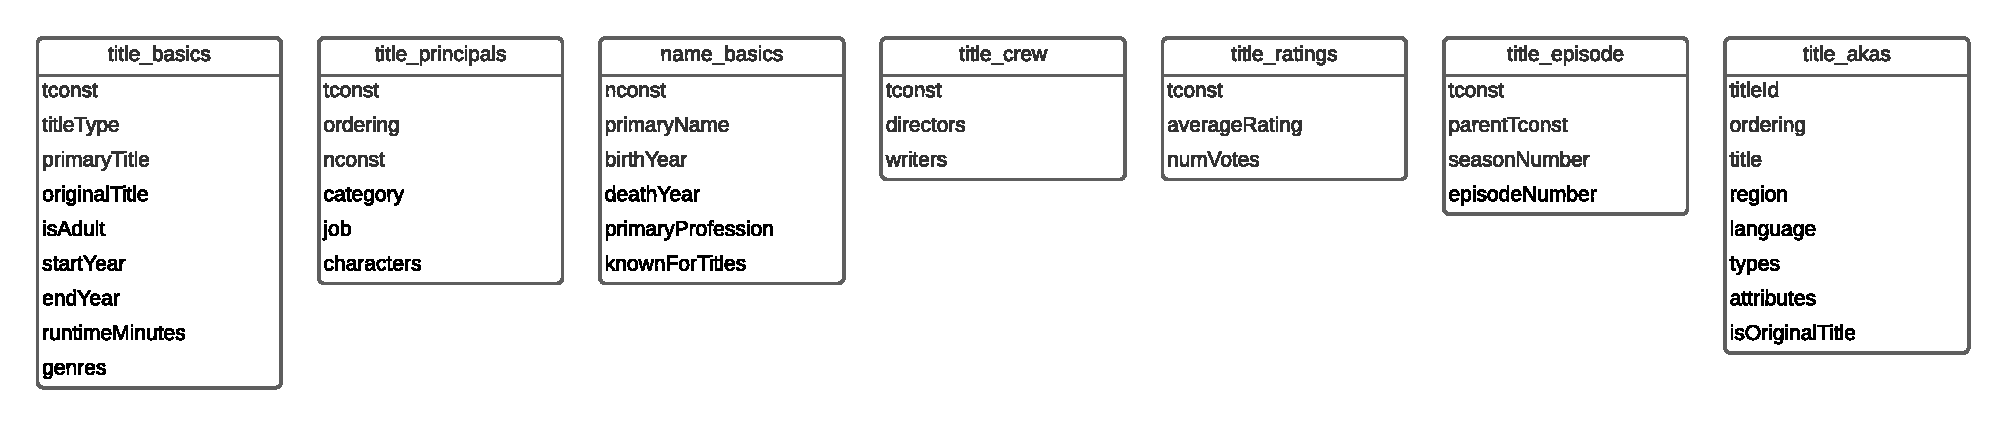
\includegraphics[width=15cm]{figures/ds.pdf}}
\end{figure}

Selected important information is stored in title\_basics and names\_basics. In the following, some first important attributes are introduced. Per title, the values of release year, runtime and genre are directly and the crew and ratings are indirectly stored and linked as entry in another database. Each person has the attributes name, birth year, death year, profession and linked titles. Rather unimportant is the data stored in title\_akas and the epsisode information in title\_episode. Any of these attributes can be analysed and compared as well as plotted over time. At later visualisations, this paper will concentrate on two types of visualisations. Numerical data such as age, time, rating and number of votes and categorial data, for example the roles, professions and genres are the first subject of comparisons. Then, time series data that combines these attributes with a time dimension will be used. 

IMDb has used and adjusted their weighted ranking $W$ for each title over the time. The current formula to calculate the score of a movie is unknown. It is based on the concept of credibility formulas used in actuarial science to deal with different types of uncertainties \citep{norberg2004}. IMDb being the largest source of motion picture data and having the largest ranking is facing malicious operations to influence the its statistics. It is known that only users who contribute on a regular basis are able to influence the ranking with their reviews. What criteria apply to IMDb's definition of a regular user however, is unknown. With $R = $ average rating, $v = $ number of votes, $m = $ minimum votes required to be listed in the top 250 (currently this attribute is 25,000) and $C = $ vote across the whole report (currently this attribute is 7), the weighted ranking once used to be $W=\frac{R*v + C*m}{v+m}$. When listing the best rated movies in the following paragraphs, a simplified ranking will be used. The best movies will be evaluated due to their average ranking with the constraint of 25,000 necessary votes and display near results to current listings on IMDb.

\chapter{Theoretical Background}
\section{Data and Information}
When approaching visualisations, it helps to understand in which context they take place. What is meant by the term data can be any raw fact without a given context. It takes a process to get information out of it. The processing can for example be structuring, ordering, searching or combining and always results in adding context to the data. The results enable decision making. Visualisations can take part in the process of gathering information from scratch data. New methods of combining, selecting, ordering and others salvage new information when applied to data. Rich contexts can be provided efficiently when using a suitable method of visualisation. 

One step further, the term knowledge often appears and relates to data and information \citep{chen2009}. \cite{ackhoff1989} defines the three terms data, information and knowledge from a perceptual and cognitive perspective. For him, data means any symbols and information refers to data that can answer the specific questions within the categories of ''who'', ''what'', ''where'' and ''when''. One step further does knowledge combine application of those two pieces and can answer ''how'' questions. In that definition, both information and knowledge are able to help making decisions, however does the complexity of knowledge exceed pure information. 

\begin{figure}[caption={The process between data and information}, label={fig:datainfo}]
	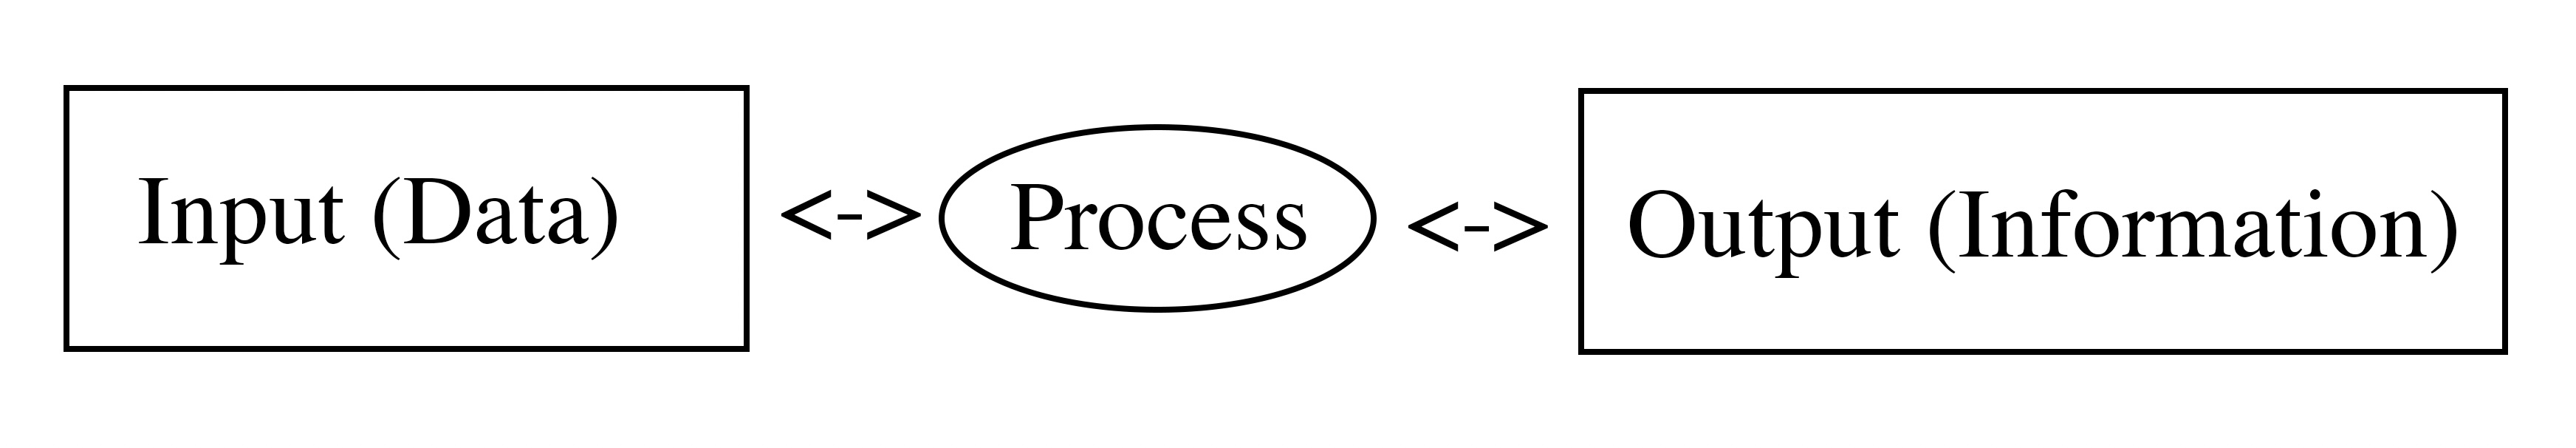
\includegraphics[width=10cm]{figures/di.jpg}
\end{figure}

Visualisations of data can deliver different information than what is usually obtained when reading out the data they rely on. The process it takes to encode the graphics and find insights is often shorter than obtaining the same results from the raw data. In some cases, the human brain is unable to discover correlations which, however can be shown easily via graphs. Figure \ref{fig:datainfo} shows that there always exists a process between information and data. This action can involve reading and understanding visualisations instead of only the data. In contrast to the encoding process, when decoding, data is converted following rules the graphic designer sets. Using computers to create figures enables new possibilities. The creator does not have to know all data points to get the results. With just knowledge of the data structure and a few selected data points, rules can be established and applied to produce results. This is especially important when the data exceeds what humans can decode in real time.

\section{Quality Criteria in Perception}

From a biological point of view, visually perceived graphics offer high bandwidths for the reception of information \citep{wilkinson2016}. When displaying multiple things, disadvantages quickly arise in cases where attention is divided \citep{cohen2016}. The ability to find patterns helps when decoding figures and is described as one of the main cognitive mechanisms \citep{keller2005}. Spatial visualisations of aggregated data allow large correlations to be identified as they provide an overview without going into every possible detail. They are distinguished from the symbolic representations of individual and precise data points.

\section*{Cognitive Fit}

\cite{vessey1991} describes the theory of the cognitive fit which can help when visualising data. The right choice of a ``Problem Representation'' can be selected with regard on the type of data. As a consequence, the ``Problem Solving Task''  appears to be easier in contrast to different representations. If task and representation fit, the resulting ``Mental Representation'' is able to work for a ``Problem Solution'' \citep [p.221]{vessey1991}. There emerges a cognitive fit when solving a problem with respect to this. Tables for example are convenient for symbolic information. They can provide precise data points and show exact data. However, when the amount of information gets too large, tables can be hard to read. Searching for information takes a long time. Also, some problems require to aggregate many information. When only using one big table, aggregating takes too long or it gets impossible. Relations between data are hard to point out and so, the cognitive fit for such tasks often is a different representation. Graphics on the other hand advocate spatial information. They can show correlations or give an overview.  In many cases, they address only certain parts or aspects of the raw data because only these are relevant to answer questions. Or they provide an overview but also go into detail regarding some aspects. This for example can be achieved by zooming in at one part of a map to enable more information in the area of interest.

\section*{Colours and Shapes}

When deciding which colours a visualisation should contain, the luminance (brightness), chroma (amount of colour) and hue (colour itself) play a role. When colours are tools to separate areas and show differences, they can be ordered in a way that fits the context of the visualization (Cognitive Fit). Brown and green tones naturally represent terrains, red and blue tones are often related to temperatures or amounts, and colours like green and red can represent positive and negative connotations. These orders can be sequential, diverging or unordered.

Shapes affect the observer in a similar manner. The shape of equally sized objects however, is harder to distinguish than their colour (if opposite colours are used). Some forms of graphs like bars and lines are easier to read for exact values than for example pie charts or plots with different rectangular areas. After deciding a fitting form of visualization and its parts, shapes can again help increase the amount of information displayed. When clustering dots in a plot for example, different shapes can indicate the  groups of data points. Next to the x- and y-axis, form, size and colour of data pints can express three additional dimensions and therefore deliver richer information.

\section*{Data-Ink Ratio}

Another aspect regarding the amount of used colour is the data-ink ratio $IR$ by \cite{tufte1983}. Described as $IR = \frac{\text{Data-ink}}{\text{total ink}}$, it shows how much of the actual ink is used to describe the data itself. All other ink should be used sparingly in order not to distract. This can involve showing axes, legendaries and additional textual descriptions. When most ink is used for the data, chances that the viewer's eye will first focus on important parts are high.

\section*{Preattentive Search}

Through preattentive search, the brain recognizes some objects or colours more than others \citep{wolfe2005}. If one colour is used only a few times, it might pop out and attract attention. With more than one channel, for example if there exist different colours and shapes, each channel will have its own extent to pop out. Colour on this matter has greater effects than the form. When mixing up many channels, distinguishing all conveyed information gets harder and slower.

\section*{Gestalt Rules}

\cite{wertheimer1923} defined several thesis that describe in which cases objects are related to each other and how their properties influence the appearance in a bigger context. The results are seven statements which should be taken into account if a visualisation is supposed to behave accordingly to the own purposes. Close (proximity), similar (similarity) and connected (connection) objects or those that share the same direction of movement (common fade) seem to belong together. Next to that, incomplete shapes are recognized as completed objects (closure) and hidden parts of objects are imaginary visualised into familiar ones (continuity). Last but not least, if there are multiple elements, in most of the cases, some will appeal to be in the foreground and others in the background (figure and ground)\citep{ali2012}.

\section{Identification of Visualisation Methods}
With varying characteristics of data, different methods for visualisations tend to suit best \citep{robertson1990}. Data can for example be scaled nominal (no order and no way to compare the quality of two values ), ordinal (can be ordered) or metric (have quantifiable distances). Next to that, the intention of the visualisation plays an important role. Some types of graphics allow for precise symbolic representation whereas others serve spatial concerns.

Typical kinds of numbers are traditionally plotted with suiting methods. Amounts are often represented in bar charts as discussed by in \cite{talbot2014}, waffle charts and heat maps. Distributions are often seen in histograms, density plots, ridge-line plots, box plots, violin plots and sina plots. Proportions can be visualised in pie charts, stacked bar charts, tree maps and nightingale charts. Associations allow for methods such as scatter plots and bubble charts. For further reading des \cite{cleveland1984b} show different facets of scatter plots. Even though there is not enough space to discuss all of these types in this paper, the most important ones as well as some special ones will be analysed. Factors that make them successful in regard of the quality criteria will be explained. Geographical data such as the topography can be drawn on maps. Different sources of maps work as foundation on top which new information can be printed. Examples are heat maps that use actual geographical maps as basis or choropleth maps. When it comes to time series, often line plots are applied. Another method of differentiating steps in time is using animations. This way, all methods above can be used and rendered multiple times with respect to changes from time to time. Many of these forms are not new and can be found and discussed in \citep{cleveland1984}.

The grammar of graphics can be used to describe the rules which apply to the creation of all the listed graphics \citep{healy2018}. It defines six aspects a plot combines. In order to visualise the following plots, the programming language R was used. Next to its orientation at data intense work, the libraries dplr, tidyverse and ggplot2 offer possibilities to clean the data with low efforts and apply the grammar of graphics to get results. Referring to the theme aspect, the library ggthemr with its theme ''dust'' was used throughout the paper. Next to the data and mapping, layers, scales, coordinate systems, facets and themes play a role. The mapping of variables to dimensions (generally visual properties) is also referred to as aesthetics. Usually, the selection of data and aesthetics is done in the first layer. Afterwords, layers can be added in order to provide additional information. A layer can consist of data, geometric objects, the mapping, statistical transformations and position adjustments. Multiple layers can for example add information like a smoothed average or divide the plot into specified facets.
 
\chapter{Comparison through Implementation} 

\section{First Visualisations}

Before comparing different methods with respect to the theoretical background, the criteria and processes following the grammar of graphics can be shown on some initial visualisations. In addition to that, a deeper insight to the data is given as these figures can be understood with regard to their data's context next to what is discussed in textual form.The IMDb contains 8,429,331 titles (as of 11th November 2021). Figure \ref{fig:imdbTitles} displays the distribution of released titles over the years whereby the year 2018 sets a peak with 405,203 units. It should be noted that the data from 2021 is not complete. The status quo of the database is before the end of 2021.

\begin{figure}[caption={Released titles per year from 1900 to 2021}, label={fig:imdbTitles}]
	{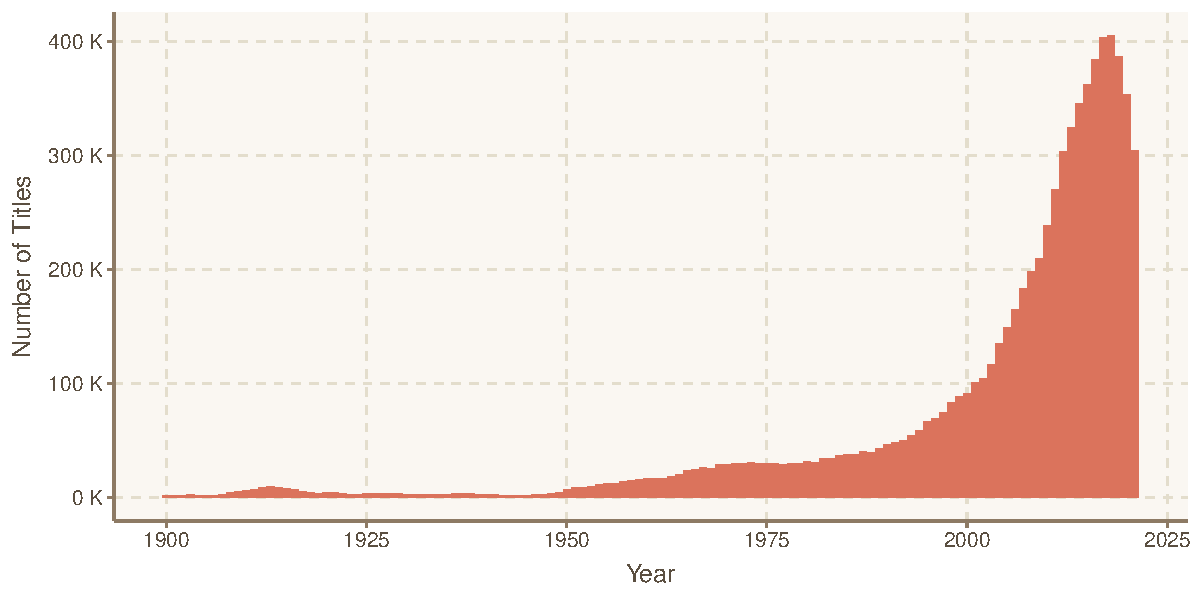
\includegraphics[width=14.5cm]{figures/titles_per_year.pdf}}
\end{figure}

In figure \ref{fig:imdbTitles} can be seen why bars suit as a method for visualising amounts. In this case one bar is used for each data point. Compared to a line diagram, as otherwise usual for time series, this can give an impression of how many years are considered. When comparing the amount of spaced used for the bars to all surrounding labels and the coordinate system, the plot's data-ink ratio is near one. The theme is not only selected in order to appeal pretty, but also prints the bars in a stronger colour than simple grey. As a result, the observer's focus is directed intentionally. 

Applying the grammar of graphics, this plot uses three layers that add up to a whole graph. The first one sets the data which has already been filtered before and sets the mapping in order to display the amounts of titles on the x-axis against the year on the y-axis. Therefore, this plot falls into the category of numerical and time series data. The next layer adds the geometric objects (bars) followed by another one to make a statistical transformation (set a continues y-axis scale). A last layer adds-axis labels.

In order to see the best rated movies, the tables title\_basics and title\_rating have to get merged by the key attribute tconst. When using the average rating and filtering for titles that are movies and have more than 25,000 ratings, the following list shows titles that are voted to be the Internet's favourites. Figure \ref{fig:imdbBest} already can be seen as a data visualisation since merging and filtering for this result is a process in order to answer a specific question. As already mentioned in the theoretical background, tables tend to suit giving precise and certain information. In this case, filtering from over eight million entries to ten entries makes the information quickly accessible.\\ 

\begin{figure}[caption={Movies with the highest average rating that contain more than 25,000 votes}, label={fig:imdbBest}]
	{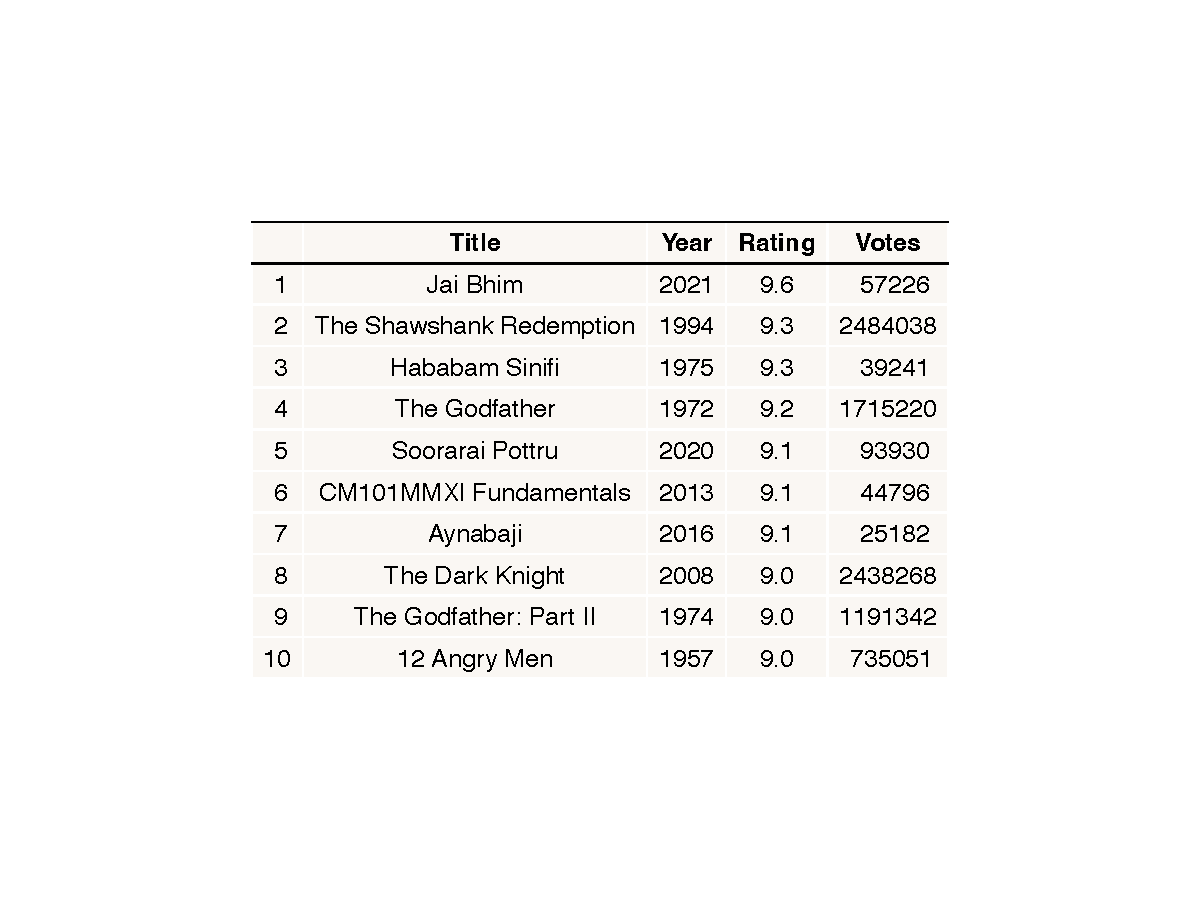
\includegraphics[width=11cm]{figures/best.pdf}}
\end{figure}

The symbolic representation in figure \ref{fig:imdbBest} correlates with IMDb's own ranking for which formula insights are not publicly available. The movies ''The Shawshank Redemption'', ''The Godfather'', ''The Dark Knight'', ''The Godfather: Part II'' and ''12 Angry Men'' also appear in the original top ten list. When asked to search for certain data, such a table can be more efficient than reading out the same data from a comparable graphic. This appears until the amount of data becomes to large and finding the right rows and columns becomes time intensive. In addition to the readability, it is hard to provide a form for a visualisation that suits the nature of the given data better that simply aligning it in a table. Even though, mapping variables to multiple dimensions is possible, it does not fit in every case.

As a third visualisation, some dimensions of the earliest movies on IMDb can de displayed. In response to the fact that figure \ref{fig:imdbTitles} does not give detailed insights on numbers of early movies because of its high y-axis scale, another graph can show richer information regarding the earliest 89 movies. The following figure \ref{fig:imdbFirst} also shows, how colour and shape are able to provide more information as introduced in a former section.\\

\begin{figure}[caption={The earliest movies listed on IMDb}, label={fig:imdbFirst}]
	{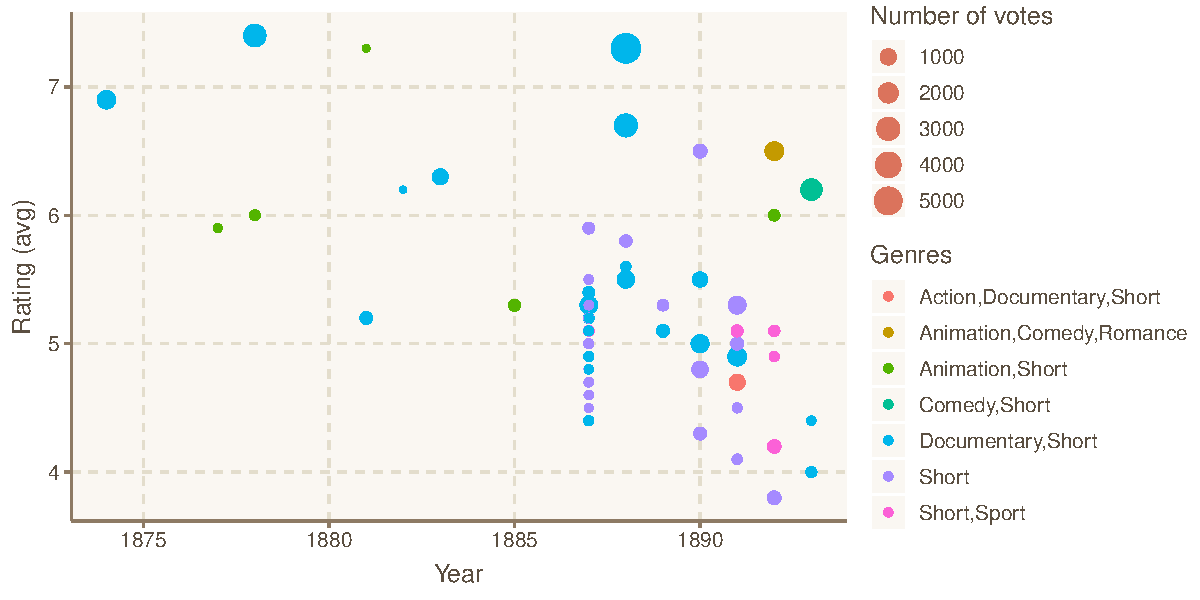
\includegraphics[width=14.5cm]{figures/first_movies.pdf}}
\end{figure}

Starting with the year and average rating on x- and y-axis, the point graph enlightens how popular movies from the years 1874 to 1893 are. It is common to plot time on the x-axis and therefore faster to read. It would seem unconventional to see the years on the y-axis and take lots of time to read. The y-axis displays the rating of the movie which indeed is the most important information, the graph contains. This dimension fits its requirements as it is  precise. Values can be clearly distinguished from each other. In addition to that, the shape shows the number of votes and the different genres are symbolised by the use of multiple colours. Objects with similar shape seem to be related as the similarity describes as one of the Gestalt rules. The colour sequence in these circumstances are unordered to show that there is no intentional relation between the different groups of genres. 

When previously talking about the correlation of data, information and knowledge as well as how they take place in real world scenarios, one now can apply the model to this graph. The raw data are symbols that represent votes, genres and much more. The process of filtering only the entries from years 1874 to 1893 and structuring it with regard to specified rules does achieve multiple outcomes. First, information is delivered when showing the year and rating of a movie. These information answer the questions of ''what'' average rating they have or ''when'' a genre was released. Second, does the graph provide a basis for deeper knowledge. The relationships of ''how'' the number of votes relates to the likelihood of achieving a high ranking, ''how'' certain years are reflected by the different genres of released movies or ''how'' the number of movies per year increases already in early stages are shown.

\section{Numerical and Categorial Data}

\section*{Amounts via regular and diverging bar charts}

Numerical data allows for visualisations of amounts, distributions, proportions and associations. In the following case, the average ratings of titles are accumulated over the whole genre. Due to the size of the database, filters had to be applied to the calculations, reducing the number of titles from over 8 million to a few tens of thousands. The graphs in figure \ref{fig:bars} examine only data points of titles from the release year 1970 (28,837 units). Since most titles are considered under multiple genres, their ratings are included in the aggregated results of all applying cases. In addition, the restriction was made that only genres that collect a minimum number of 120,000 votes are considered. This avoids outliers with only a few votes, which would otherwise distort the visualizations. 

\begin{figure}[caption={Best voted genres in 1970 via diverging (left) and  regular bar chart}, label={fig:bars}]
	{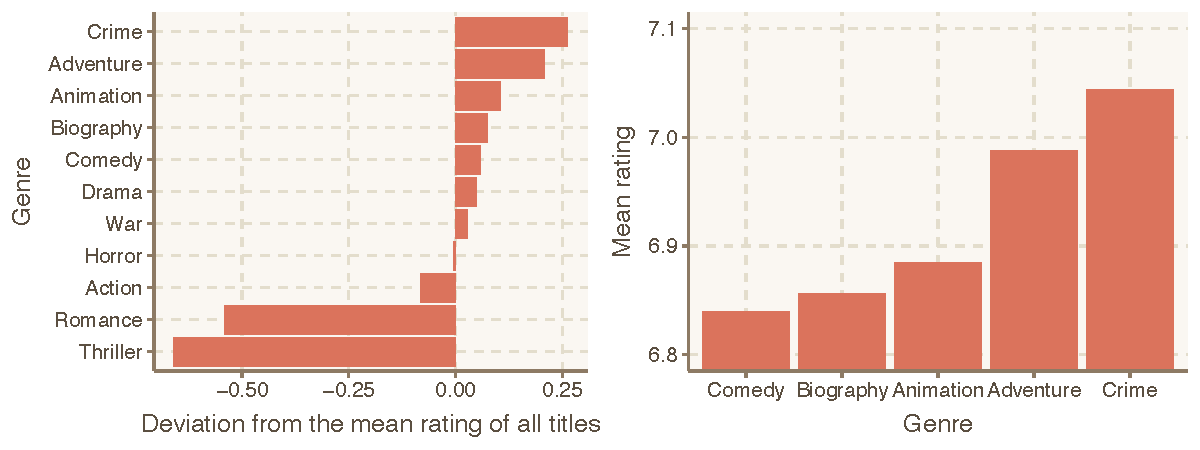
\includegraphics[width=14.5cm]{figures/bars.pdf}}
\end{figure} 

Both graphs correspond to a cognitive fit that satisfies a question about the ratings of individual genres. The shape of the bars is suitable for making different ratings comparable. Also, a similar amount of ink is used in both graphs providing a decent data-ink ratio. In both cases, the Gestalt rules can be acknowledged to provide a connection of different characteristics. Comparatively long bars seem to convey a connection. However, the differences already start with the proximity. In comparison, the distances in the left visualisation are emphasized more strongly by the fact that the bars swing in two directions.

Differences arise when looking at the arrangement of the variables on the x- and y axis. In the normal bar chart, the categorical data (genres) are shown on the x-axis. Their values can be efficiently read from the y-axis. The diverging bar chart, however, takes a different approach. Here the coordinate axes are swapped. The result is that more categories can be mapped compared to the right side. The width of the bars has no significance here, in contrast to e.g. histograms, and can therefore be adjusted. The division on the x-axis has the effect that the rating itself is no longer in the foreground, but the distance from the average rating of all genres can be read off. The graphic on the left thus provides an overview of how the individual genres compare to the average. It is clear that the negative gap between the action and romance genres is weighted more heavily than the positive advantages of the above-average genres.

\section*{Proportions via pie chats and treemaps}

The next discipline for visualizations are proportions of variables. In the following, the individual activities of the principles are recorded and put into a size comparison. Again, the limitations are to be explained first. As data basis all entries of the database title\_principals are used, which contains 47,576,376 rows. Since it is not necessary to operate on the data, but only rules for structuring are applied, no further selection must take place here. However, the categories ''self'', ''archive\_sound'' and ''archive\_footage'' were sorted out, since they do not offer any conclusion on professions.

\begin{figure}[caption={Porportions of prefessions via pie chart (left) and treemap}, label={fig:prop}]
	{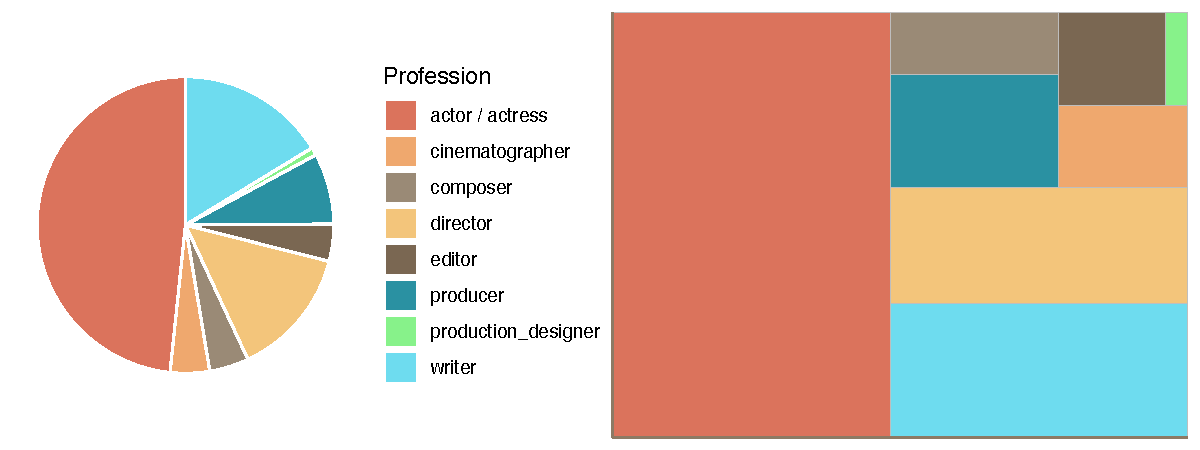
\includegraphics[width=14.5cm]{figures/prop.pdf}}
\end{figure} 

Subsequently, the theoretical criteria can again be applied to the solutions. Both graphs fulfill a cognitive fit by answering the question of proportions with the same mean. For a simple comparison of proportions, the areas of the individual fields can be used. Problems with the pie chart occur at moments when surfaces do not have large differences in their volume \citep{schonlau2008}. For example, the difference between the characteristics of cinematographers and composers cannot be read exactly on the pie chart. The treemap cannot show the differences exactly either, since the width and height of the areas differ. But the mapping of especially small parts by rectangles works better. The area of the production\_designr is better to recognize than with the pie chart. It can be said that these types of graphs work out for spatial information rather then symbolic representation. Precision is not guaranteed however, a broad understanding of the size of components is delivered.

\section{Time Series Data}

Time series data can shed light on history. Since this is based on release years of more than the last 100 years, conclusions can be made about the past. The following graphics are about series. Each drawn point represents an example. First the release periods in years and then the running times in minutes are compared. In both cases, two facets are used to separate series from short series. In this way, differences can be shown. 

\begin{figure}[caption={Periods of broadcasting series}, label={fig:dur}]
	{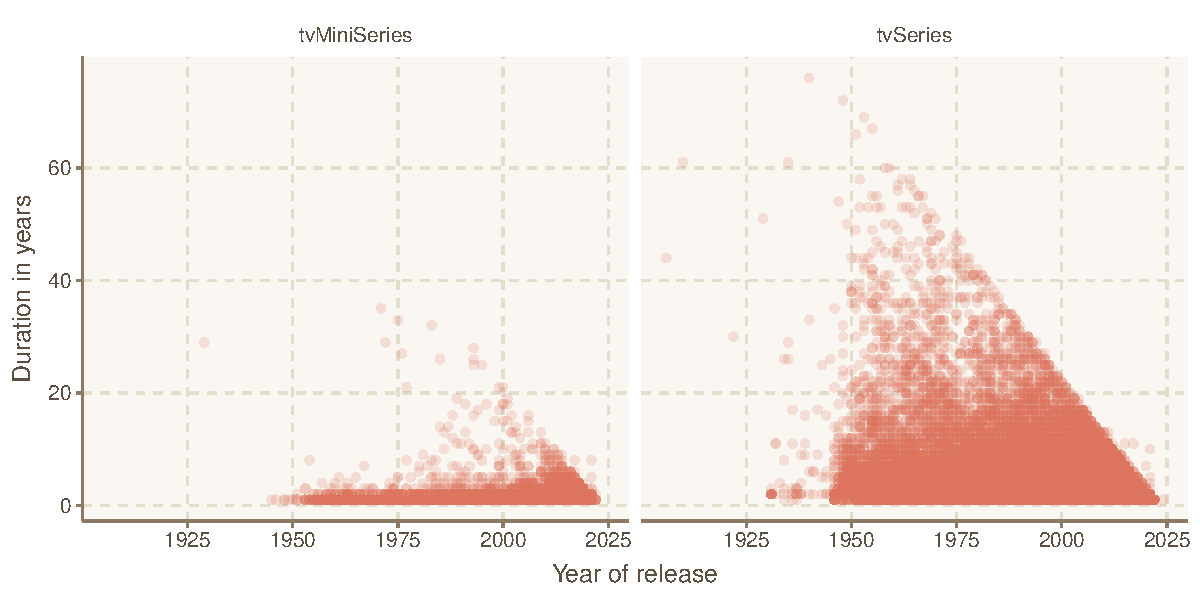
\includegraphics[width=14.5cm]{figures/ts_dur.pdf}}
\end{figure} 

With regard to the time periods of the broadcasts, it is noticeable that short series have fewer entries that have appeared for significantly longer than 20 years. The slanted line, which is particularly evident in the regular series, shows those series that are still being broadcast today. The oldest surviving series date back to before 1950. Due to the adjusted alpha values (transparency) and according to the principles of preattentive search, the viewer's attention is directed to those areas that have particularly intense color tones and thus many close entries. Despite the same structure and distribution of both figures, it must be pointed out that the y-axes are linear in one case and logarithmically scaled in the other case.

Furthermore, the runtime of the series can be recorded. Some stripes are displayed, which mark often selected run times like e.g. 40 minutes. Many series are rated with a running time of around 60 minutes, which plays off an episode length. Others have a running time of well over 10 hours, which alludes to the fact that some runtimes are recorded as total runtimes, whereas most reflect a running time that corresponds to the scale of an episode. In both cases, a similar swing around 60 minutes can be seen. The distributions appear to be distributed around it like a bell curve. Note, however, that the y-axis is logarithmically scaled. This has the effect that a few extreme values distort the scaling in such a way that the rest is not adequately represented.

\begin{figure}[caption={Runtimes of series}, label={fig:min}]
	{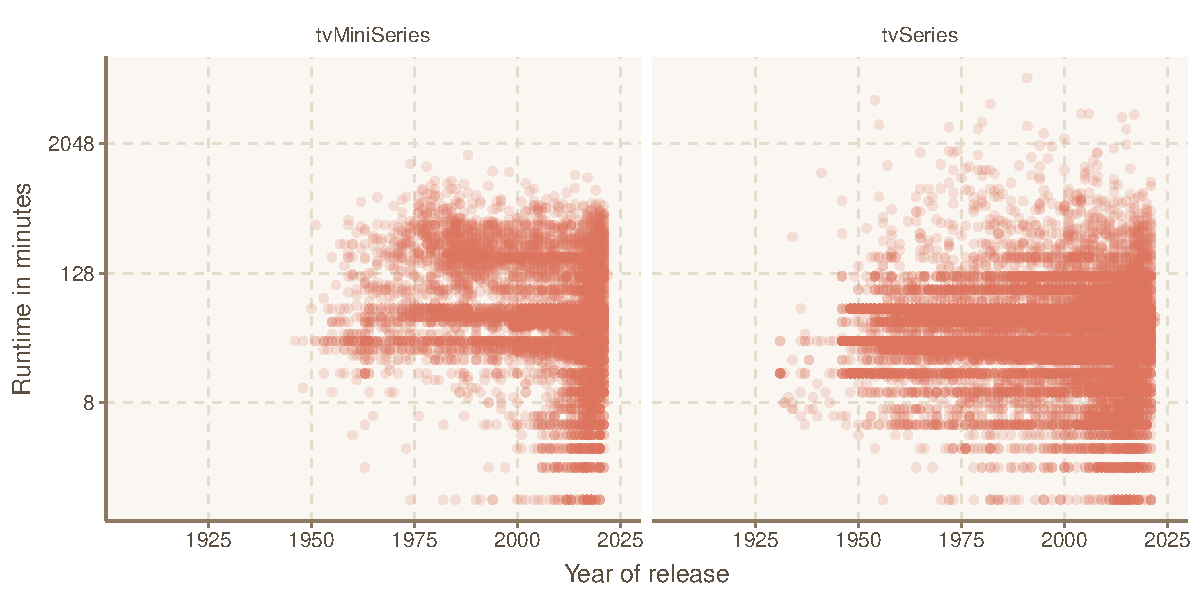
\includegraphics[width=14.5cm]{figures/ts_min.pdf}}
\end{figure}  

Recapitulating, the theoretical basics can be applied here as well. In terms of shapes, the individual circles represent the individual data points. The transparency allows statements about the density of the individual observations, so that patterns, where many occurrences lie, are noticeable. The Gestalt rules can be applied here multiple times. On the one hand, the shapes are close to each other, on the other hand, they do not necessarily have the same color in every situation, but express a connection through their transparency (hue). Weak colors can be distinguished from those that are stronger.

\chapter{Conclusion}

\section{Evaluation of Findings}

After some criteria for the examination of graphs have been established, methods for their production have been listed, and concrete examples have been used to illustrate the effects mentioned, results can now be written. There are some rules and basics that good visualizations follow. They avoid that unimportant elements attract attention, that information is conveyed falsely or that impressions are awakened that do not correspond to the actual context.

Various guidelines such as the Data-Ink ratio and the Gestalt rules can be followed in order to display the information contained in the data as efficiently as possible. For a broader understanding can be derived from the models of the cognitive fit, preattentive search and the relationship between data, information and knowledge. Being aware of the effects that colors and shapes have on the observer is a final elementary building block on the way to successful graphics.

Subsequently, if the theoretical principles are observed, the choice of visualization environment can make significant differences. Computer interfaces that do not require manual input of commands and are managed via visual buttons offer convenient solutions for taking the first steps. But if you want to work with almost no restrictions when creating graphics, programming languages provide a more suitable option. With its many available libraries, the free and statistically oriented programming language R offers a platform that is difficult to compete with for others. The libraries ggplot2,  tidyverse, dplyr, treemapify and many more allow for a procedure that follows the grammar of graphics. With several layers data can be entered, properties can be changed and elements can be added. For example, these layers have been used to split graphics into facets, change axis scales, assign additional dimensions to individual variables, and much more.

Results of the practical work are, among others, that bar-, point-, pie charts and treemaps are suitable to convey spatial relationships. Within this list, bar charts and point charts are more precise than pie charts and treemaps. However, they focus on different types of data as a broad understanding of the the information conveyed can be delivered faster by the less precise methods. Tables fulfil the purpose of accuracy, but cannot be inferred at a moment's notice. Their representation type fits symbolic data and can be especially useful when the amount of information does not exceed what can be printed readable onto one page.

\section{Further Implications}

Further implications involve the perception of the surrounding world. Judged by the above criteria, some well-known visualizations appear in a bad light, while others stand out positively from the crowd.

For example, it can be explained why the German Tagesschau refrains from showing election results by means of pie charts. This form serves excellently for the representation of proportions of a whole and is also not uncommon for comparable situations. Nevertheless, the areas cannot be read off exactly in terms of their percentages. Bar charts seem less suitable for depicting the composition of a whole, but they are more accurate.

Visualization is something everyone encounters in everyday life. Especially in times when statistics from various sources have an influence on our lives, it is even more important to be critical towards graphs that do not show common quality features. This can be the case, for example, if the axis distances do not run linearly or logarithmically, but run arbitrarily.

\section{Outlook}

Finally, reference should be made at this point to limitations, open possibilities and further questions. Due to the amount of data and the calculation times, reduced data sets with 3,000 instead of many million rows were used to create the graphs. For the final creation all original data sets were used. Nevertheless, there were cases in which individual time segments were considered instead of the entire period for faster calculation. With more time, computing power and more efficient instructions, more meaningful visualizations can be created here.

Other possibilities also arise in relation to the use of data and the use of criteria and models from the literature. Further processing of the data and application of additional methods can reveal new references to criteria. On the basis of further theories, additional statements can be made and existing graphs can be viewed in a new light. Viewing of geographic data or with possibilities of animation and interaction with graphics offers a prospect on not treated topics that are worth exploration.

Further papers on the subject of IMDb that not necessarily focus on data visualisation and for example focus on sentiment analysis are among others written by \cite{dodds2006}, \cite{kumar2019}, \cite{oghina2012}, \cite{yenter2017} and \cite{otterbacher2012}.